\documentclass[11pt]{article}
\usepackage{ctex}
\usepackage{graphicx}
\usepackage{algorithm}
\usepackage{algorithmic}
\usepackage{amssymb}
\usepackage{amsmath}
\usepackage{hyperref}


\begin{document}
\title{马氏链蒙特卡洛方法的应用}
%\subtitle{概率论与随机过程(2)  第一次大作业}
\author{无47\hspace{2em}刘前\thanks{清华大学电子工程系(E-mail: liuqian14@mails.tsinghua.edu.cn)}\hspace{2em}2014011216\hspace{2em}}

\maketitle


\begin{abstract}
  本文第一部分,以马氏链蒙特卡洛(Markov Chain Monte Carlo, MCMC)方法中的Metropolis-Hastings(MH)算法为基础,深入全面地讨论了MH算法中提议函数(proposal function)的参数选择、随机样本的选取方法等问题,逐步优化估计结果,使其尽量与真实参数相近,得到了一些令人满意的结果。另外,本文还介绍了一种针对于提议函数参数选择的自适应算法,讨论了算法的可行性。同时,使用MH算法的特例Gibbs采样法,得到质量更高的随机样本。该部分通过生成给定二维高斯分布的随机样本,对算法进行了测试,结果表明,优化后的MH算法生成的随机样本对相关系数估计的精确度和稳定性比优化之前明显更高。
  
  本文第二部分实现了AIS,TAP(包括二阶近似和三阶近似)和RTS三种采样算法,对四种受限玻尔兹曼机(RBM)模型的归一化常数进行了估计,并尝试讨论了算法参数对估计结果的影响,将三种算法的性能加以对比。同时还尝试使用对比散度(CD)算法重新训练了RBM模型,在训练模型上进一步估计归一化常数。
\end{abstract}


\newpage
\begin{center}
\tableofcontents
\end{center}
\newpage


\section{背景介绍}
马尔科夫链蒙特卡洛(Markov Chain Monte Carlo, MCMC)方法,从1950年萌芽,在实践中不断发展,被广泛应用于各学科领域(如信息科学、物理、化学、生物学、金融、材料等)的科学计算\cite{UMH},并且随着机器学习和深度学习的流行,日益展示出其强大的影响力。

MCMC方法常用于模拟复杂的非标准的多元分布,生成服从复杂分布的随机样本,其中最重要的一种方法是Metropolis-Hastings(MH)算法,最早由Metropolis,Rosenbluth等人提出并发展\cite{MH1}。MH算法用处十分广泛,著名的Gibbs采样算法也只不过是MH算法的一个特例\cite{Gelman}。尽管MH算法已经被提出四十余年,但是仍然有很多学者在研究这一算法。比如,Bishop指出了MH算法在模式识别和机器学习领域的广泛应用\cite{PRML},同时Jun S. Liu也指出了MH算法在科学计算的作用\cite{Jun},从中可以看出MH算法在最前沿的课题中仍然意义重大。

本文从MCMC算法出发,主要分为两部分内容:PART A将使用MH算法对给定的二维高斯分布进行随机采样,并根据生成的样本估计相关系数。为了提高相关系数估计的准确度,文中尝试对MH算法中各种参数的选择进行了系统而深入地讨论。PART B将使用三种不同的采样算法对四种RBM模型(隐变量分别为10,20,100,500)进行归一化常数的估计,并根据估计值计算出不同模型在测试数据上的似然值,也尝试对算法进行了进一步的分析讨论。

\section{Part A: Metropolis-Hastings算法应用}
\subsection{背景介绍}
Metropolis-Hastings算法是一种重要的随机样本生成方法,然而一般的MH算法没有对提议函数及其参数的选取给出明确的方法,同时对随机样本间的独立性也没有强制要求。\cite{MH_A}对提议函数及其方差的选取对采样结果的影响作了基础的讨论,并由此推出一种改进的自适应算法用以寻找正态型提议函数的方差,一定程度了提高了算法的可控性,但是无法保证随机样本间的独立性,因而本文还尝试通过检验生成的随机样本的自相关系数,给出了选择独立性较高的随机样本的方法,从而实现随机样本更接近真实分布。


\subsection{Metropolis-Hastings算法}

设$\pi=(\pi(i)>0,i\in S)$为任意给定的概率分布,$\mathbf{T} = (T(i,j),i,j\in S)$为选择的易于实现的条件概率转移矩阵$(T(i,j)>0,i,j\in S)$(称$\mathbf{T}$为参照矩阵)。$X= \{X_{n},n\geq 0\}$由下列步骤生成\cite{Lin}:

(1) 给定$X_{n}(X_{n}\in S,n\geq 0)$,根据$\mathbf{T}(X_{n},\cdot )$抽取$Y$;

(2)计算得到接受概率(Accept Probability),计算公式为:
\[p(X_{n},Y)=min\{1,\frac{\pi(Y)\mathbf{T}(Y,X_{n})}{\pi(X_{n})\mathbf{T}(X_{n},Y)}\}\]

(3) 抽取$U\sim U[0,1]$,如果 $U<p(X_{n},Y)$,则令$X_{n+1}=Y$,否则$X_{n+1}=X_{n}$。返回步骤(1)。

由上述步骤生成的$X=\{X_{n},n\geq 0\}$是不可约马氏链,其平稳分布即为给定概率分布$\pi$。

Metropolis-Hastings算法可以总结为Algorithm\ref{alg_MH}。
\begin{algorithm}[t]
\caption{Metropolis-Hastings算法} 
\textbf{输入:} 概率分布密度$\pi(x)$;条件概率转移矩阵$\mathbf{T} = (T(i,j),i,j\in S)$;生成的随机样本数$N$;

\textbf{初始化:} $X_{1}$

\textbf{输出:} $X=\{X_{n},n\geq 0\},n=1,2,\cdots,N$

\textbf{for} $n=1:N-1$ 
\begin{enumerate} 
  \item 由$\mathbf{T}(X_{n},\dot)$抽取$Y$;
  
  \item 计算接受概率(Accept Probability):
\[p(X_{n},Y)=min\{1,\frac{\pi(Y)\mathbf{T}(Y,X_{n})}{\pi(X_{n})\mathbf{T}(X_{n},Y)}\}\]

  \item $U\sim U[0,1]$,如果 $U<p(X_{n},Y)$,则$X_{n+1}=Y$;
  
  否则$X_{n+1}=X_{n}$。
\end{enumerate} 
\textbf{end} 
\label{alg_MH}
\end{algorithm}

\textbf{注意:} MH算法中的条件转移矩阵常常是一个辅助的概率密度函数(提议函数),记作$q(x,y)$。同时,为了保证随机样本确实符合平稳分布(目标分布)$\pi(x)$,常常选取$n$足够大之后的随机样本。

\subsection{Metropolis-Hastings算法的深入讨论}
\subsubsection{问题描述}
给定二维高斯分布,
\begin{figure}[h]
    \centering
    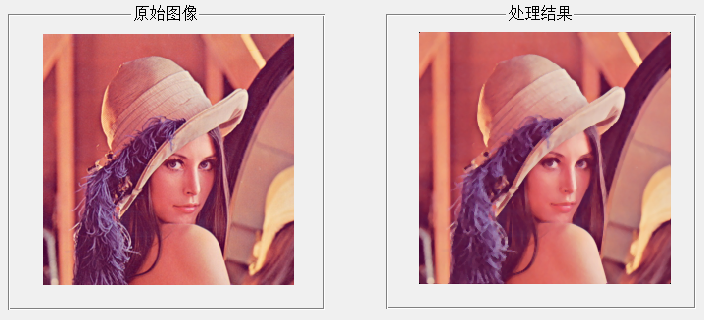
\includegraphics[scale=0.4]{gauss.png}
    \caption{目标分布(二维高斯分布)}
  \end{figure}

要求使用Metropolis-Hastings算法对该分布进行随机采样,并使用生成的随机样本估计该二维高斯分布的相关系数。事实上,很容易得出该二维高斯分布的相关系数为0.5。

根据对MH算法的描述,可以看出算法中不确定的因素有很多,因而在实现算法之前,需要解决以下几个问题,包括:

(1) 如何选取迭代初值;

(2) 如何选取提议函数$q(x,y)$(包括提议函数自身的参数);

(3) 需要生成多少随机样本;

(4) 随机样本在$n$至少为多大才能保证已经收敛到平稳分布;

(5) 提高随机样本独立性的具体方法;等。

这些因素都会对MH算法的性能造成一定的影响。下文将逐一解决这些问题。

\subsubsection{迭代初值的选取}
MH算法保证了只要迭代初值在分布函数定义的区间内,最后将会收敛到目标分布,因而,在选取迭代初值时可以不必太纠结。一般选取生成随机数的方法,可以帮助解决初值选取的困难。

对于\textbf{问题描述}中的二维高斯分布,$X_{1}$和$X_{2}$可以使用均匀分布或者一维高斯分布生成随机样本。使用均匀分布时,可以先限定一个大致范围,范围的选取可以根据目标分布的均值来选择;使用一维高斯分布时,均值可以选择目标分布的均值,方差任选。

总之,MH算法中迭代初值的选取比较随意,对算法的最终结果不会造成很大影响,但对算法的运行效率影响较大。

\subsubsection{提议函数的选取}
MH算法中对提议函数$q(x,y)$的选取没有给出特别的要求,因而从理论上说,提议函数$q(x,y)$的选取可以是任意的。但是,实际中需要考虑到算法实现的难易程度以及算法的运行效率,因而选取提议函数$q(x,y)$需要多加一些考虑。

一般认为,提议函数至少需要满足以下两个要求\cite{MH_A}:

(1)对于固定的$x$,能够便捷地从$q(x,y)$中产生随机数。

(2)提议函数形式与目标分布越接近,生成的随机样本效果越好。

对于\textbf{问题描述}中的二维高斯分布,满足上面要求的最佳函数$q(x,y)$即为一维高斯分布,既满足方便生成随机数的要求,而且与目标分布很接近。同时,一维高斯分布还有一个突出的优点是具有对称性,也就意味着在计算接受概率时,计算公式可以简化为:

\[p(X_{n},Y)=min\{1,\frac{\pi(Y)\mathbf{T}(Y,X_{n})}{\pi(X_{n})\mathbf{T}(X_{n},Y)}\}=min\{1,\frac{\pi(Y)}{\pi(X_{n})}\}\]

综合以上特点,$q(x,y)$选取以$x$为均值的一维高斯分布。

但是问题随之而来,一维高斯分布的均值与方差如何确定?

\cite{MH_A}中使用随机游动的方法,均值选择为当前的状态$X_{n}$,对于方差则提出了一种寻找提议函数方差的自适应算法Algorithm\ref{alg_APMH},让接受概率落入一个可以接受的范围,以此为判断条件找到合适的方差值。

\begin{algorithm}[t] 
\caption{高斯形式提议函数的方差的自适应Metropolis-Hastings算法} 
\textbf{输入:} 高斯分布的提议函数$N(X_{i},\sigma_{n})$;接受概率的置信区间$[a-\epsilon,a+\epsilon]$;引入另一个方差$\hat{\sigma}$;操作次数$N$;每次生成的Markov链长度$M$

\textbf{初始化:} $\sigma_{0}=0,n=0$

\textbf{输出:} $\sigma_{n},n=0,1,\cdots,N-1$

\textbf{for} $n=0:N-1$ 

\begin{enumerate} 
  \item 根据提议函数$N(X_{i},\sigma_{n})$,采用随机游动采样法生成一条长度为$M$的Markov链;
  
  \item 计算第1步中产生的Markov链接受新状态的比率$P_{n}$;

  \item 若$P_{n}\in[a-\epsilon,a+\epsilon]$,则令$\sigma=\sigma_{n}$,退出算法;否则继续执行下一步;

  \item 若$n>2$且$\vert P_{n}-a\vert<\vert P_{n-1}-a\vert$,则置$\sigma_{n}=\sigma_{n-1}$;

  \item 从$N(\sigma_{n},\hat{\sigma})$产生一个随机数,记作$\sigma_{n+1}$;

\end{enumerate} 
\textbf{end} 
\label{alg_APMH} 
\end{algorithm}

从Algorithm\ref{alg_APMH}描述中可以看出,为了获取一个较为合适的方差值进行了复杂的操作,引入了额外的计算负担,同时在算法中又引入了新的方差参数$\hat{\sigma}$,而$\hat{\sigma}$的选取又带来了新的问题。因而这一算法的提出可能更多停留于理论层面,在实际应用中还要考虑到该算法带来的计算效率降低的问题。

至此,提议函数$q(x,y)$的选取问题基本得到了解决。

\subsubsection{生成随机样本的数目}
\textbf{问题描述}中需要根据生成的随机样本估计目标分布中的相关系数,为了提高对相关系数估计的准确性,必须得到足够数量的随机样本。通过后面的仿真部分,可以基本得出随机样本数目越大,对目标分布参数的估计越精确的结论,效果越好。但在实际应用中,随机样本数不是越大越好,因为随机样本数目的增加会造成计算量和计算时间的增加,因而应该根据实际需要在估计精度和计算效率之间加以平衡。

\subsubsection{判断随机样本收敛到目标分布}

MH算法生成的随机样本$X_{n}(X_{n}\in S,n\geq 0)$中只有当$n$足够大时,才能保证此时生成的随机样本收敛到目标分布(或者说与目标分布十分接近)。为了使得估计的相关系数与真实值更加接近,通常情况下,可以人为选择靠后生成的随机样本,虽然不能保证已经收敛到目标分布,但是已经能够满足实际应用的要求。事实上,如果判断随机样本与目标分布是否收敛,往往需要增加一些附加的运算和判断条件,从而降低算法的效率,这是得不偿失的。因而,本文采取普通的方法:选取靠后生成的随机样本,不对这一问题做特殊的处理。

\subsubsection{提高随机样本独立性的具体方法}
Bishop在\cite{PRML}中指出,MH算法生成的连续的随机样本是高度相关的,这与我们生成独立同分布的随机样本的目的相悖。为了更好地保证得到独立的随机样本,常常需要间隔选取随机样本,当间隔足够大时,所得的随机样本之间的独立性就会非常好。

随机样本间的独立性可以用自相关系数来衡量\cite{MH_A},自相关系数绝对值越小,说明随机样本序列之间的相关性越弱,独立性越强。在后面的仿真中,针对生成二维高斯分布随机样本的问题,作出自相关系数随采样间隔变化的关系,可以看出间隔在一定范围内增加时,样本自相关系数绝对值会明显降低,表明样本间独立性明显提高;但是当间隔继续增加时,可能会呈现出上下摆动变化的情况,因而随机样本间的独立性并不严格随着间隔的增加而减弱。

总之,根据随机样本的自相关系数来选择采样间隔,能够有效提高随机样本的独立性。

\subsection{Metropolis-Hastings算法仿真(Simulation)与优化}
下面将通过仿真(Simulation)得到数值结果,对上面关于MH算法的详细分析作直观地展示。本文中所有仿真结果均在Windows 8.1操作系统、使用MATLAB R2014a进行仿真得到。

\subsubsection{提议函数方差的选择}

\noindent\emph{仿真的基本参数设置}

a) 初始值由均匀分布随机生成,$X_{1}$的初值由[0,10]之间的均匀分布生成,$X_{2}$的初值由[0,20]之间的均匀分布生成;

b) 随机样本数量均设定为10000,选取后5000个(不间隔选取)用于估计目标分布的相关系数;

c) 独立运行次数为100次,用于观察估计值的精确度和稳定性。

在以上设定下,提议函数采用一维高斯的随机游动方法,$X_{1}$和$X_{2}$的方差(分别记作psigma1\footnote{表示proposal function的方差}和psigma2)均为三组0.5、1、2,相互组合共有九种情况。图\ref{MH_Sigma}比较了不同方差下的运行结果。

根据图\ref{MH_Sigma},不同的(psigma1,psigma2)组合估计得到的相关系数结果差异很大,只有(psigma1,psigma2) = (1.0,1.0)的估计值相对集中在精确值0.50附近,精确度相对高一些,但是数值上仍然有很大的波动,因而估计的结果稳定性很差,仍需要进一步的优化。

\begin{figure}
\begin{minipage}[t]{0.5\linewidth}
    \centering
    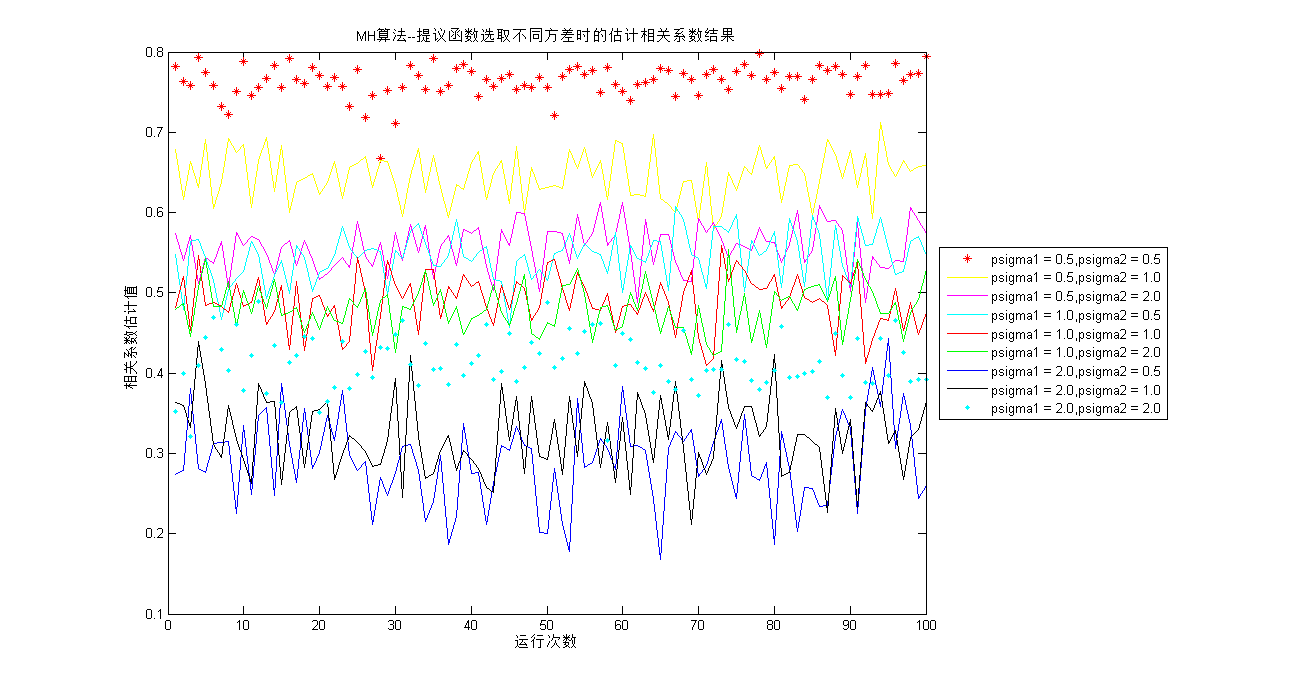
\includegraphics[width=7.0cm,height=5cm]{MH_Sigma.png}
    \caption{\scriptsize{提议函数选取不同方差时对相关系数的估计}}
    \label{MH_Sigma}
\end{minipage}
\begin{minipage}[t]{0.5\linewidth}
    \centering
    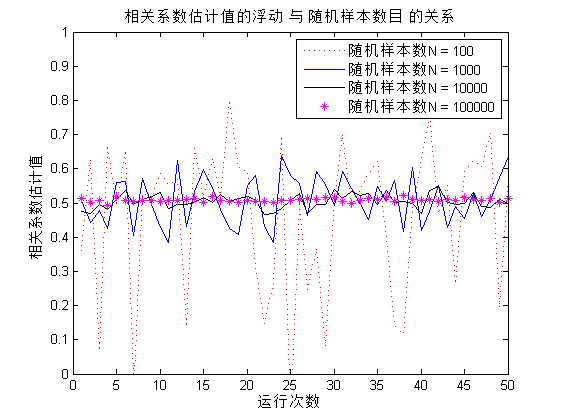
\includegraphics[width=6cm,height=5cm]{MH_Sample_Num.png}
    \caption{\scriptsize{随机样本数目不同时对相关系数的估计}}
    \label{MH_Sample_Num}
\end{minipage}
\end{figure}

\subsubsection{随机样本数目的选择}

\noindent\emph{仿真的基本参数设置}

a) 初始值由均匀分布随机生成,$X_{1}$的初值由[0,10]之间的均匀分布生成,$X_{2}$的初值由[0,20]之间的均匀分布生成;

b) 提议函数采用一维高斯形式,$X_{1}$和$X_{2}$的方差均为1;

c) 独立运行次数为50次,用于观察估计值的精确度和稳定性。

随机样本数量分为100,1000,10000和100000四组,不间隔选取随机样本,图\ref{MH_Sample_Num}比较了随机样本数量不同的情况运行结果。

图\ref{MH_Sample_Num}直观地展示出,随机样本数不同时,估计得到的相关系数结果差异很大。随着随机样本数目的增加,估计得到的相关系数明显越来越精确和稳定,当随机样本数达到10000时,可以看出相关系数估计值基本稳定于精确值0.50附近。

\subsubsection{对随机样本间隔的选择}

\noindent\emph{仿真的基本参数设置}

a) 初始值由均匀分布随机生成,$X_{1}$的初值由[0,10]之间的均匀分布生成,$X_{2}$的初值由[0,20]之间的均匀分布生成;

b) 提议函数采用一维高斯形式,$X_{1}$和$X_{2}$的方差均为1;

c) 独立运行次数为50次,用于观察估计值的精确度和稳定性;

d) 用于估计相关系数的随机样本数均为10000(生成的随机样本总数不同)。

图\ref{MH_Step}直观地展示出,选取不同间隔的随机样本时,估计得到的相关系数结果差异也比较大。随着间隔的增加,估计得到的相关系数明显更精确,稳定性也更高。

\begin{figure}
\begin{minipage}[t]{0.5\linewidth}
    \centering
    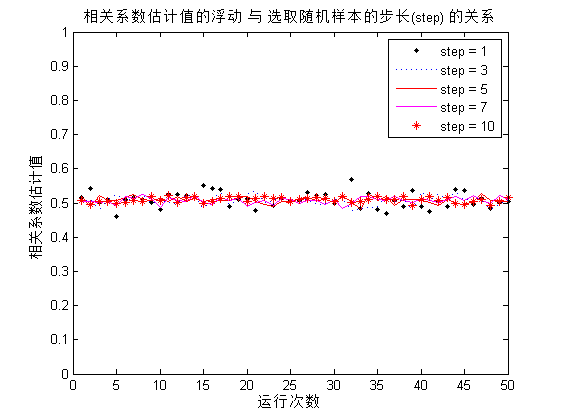
\includegraphics[width=6.5cm,height=5cm]{MH_Step.png}
    \caption{\scriptsize{随机样本间隔不同时对相关系数的估计}}
    \label{MH_Step}
\end{minipage}
\begin{minipage}[t]{0.5\linewidth}
    \centering
    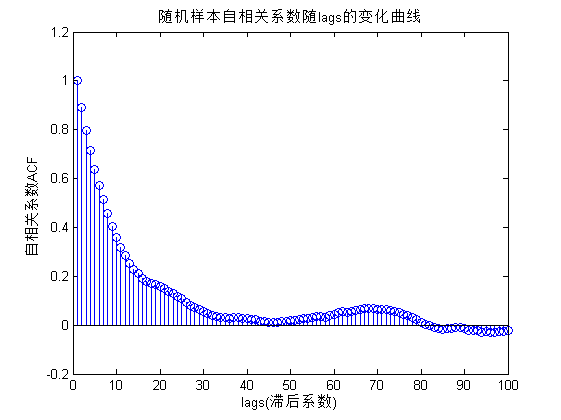
\includegraphics[width=6.5cm,height=5cm]{MH_AutoCorr.png}
    \caption{\scriptsize{随机样本自相关系数随间隔的变化}}
    \label{MH_AutoCorr}
\end{minipage}
\end{figure}

事实上,从随机样本的自相关系数角度,也能得到类似的结论。使用MATLAB R2014a的autocorr函数对生成的随机样本进行分析。图\ref{MH_AutoCorr}体现了随机样本的自相关系数与lags(滞后系数)的关系,本质上体现了间隔不同时选取的随机样本的独立性。可以看出,lags越大,自相关系数越小,因而间隔越大,随机样本间的独立性越高。

\subsubsection{参数优化后的MH算法}
经过上述对MH算法参数的深入讨论,可以得到一个针对二维高斯分布进行了参数优化的MH算法,优化后的参数设置如下:

a) 初始值由均匀分布随机生成,$X_{1}$的初值由[0,10]之间的均匀分布生成,$X_{2}$的初值由[0,20]之间的均匀分布生成;

b) 提议函数采用一维高斯形式,$X_{1}$和$X_{2}$的方差均为1;

c) 选取随机样本的间隔为10;

d) 用于估计相关系数的随机样本数均为10000,意味着共生成100000个随机样本。

之后\textbf{数值结果与算法比较}中所指的“参数优化后的MH算法”,采用上述参数进行仿真。

\subsection{Gibbs采样算法}
\subsubsection{背景介绍}
在之前实现Metropolis-Hastings算法的过程中,不难发现,MH算法的一个突出缺点是对提议函数的选择和调整比较复杂,有时还会掺杂着一些主观猜测的成分,给实际应用带来了一定的困难,而这些问题可以通过Gibbs采样得以解决。通过后面分析可以看出,在使用Gibbs采样方法时,不需要认为反复调整提议函数的形式;同时,Gibbs采样接受了所有生成的随机样本,因而生成随机样本的效率得到明显提高\cite{Jun}。

\subsubsection{算法描述}
为了方便地解释Gibbs采样算法,以二维分布为例,现要生成服从联合分布$f(\theta_{1},\theta_{2})$的二维随机样本。

使用Gibbs采样算法的前提是已知二维分布的联合分布。根据二维联合分布$f(\theta_{1},\theta_{2})$,可以得到$\theta_{1}$和$\theta_{2}$的条件分布$f(\theta_{1}\vert\theta_{2}=\theta_{2}^{(t)})$以及$f(\theta_{2}\vert\theta_{1}=\theta_{1}^{(t)})$。得到以上条件分布之后,即可采用Gibbs采样算法对二维分布进行采样。

首先,对样本进行初始化,得到$\theta_{1}^{(1)}$和$\theta_{2}^{(1)}$,并且设定迭代次数$T$。然后开始迭代生成随机样本,每次迭代的过程与MH算法类似。在第t次迭代时,根据$f(\theta_{1}\vert\theta_{2}=\theta_{2}^{(t-1)})$生成随机样本$\theta_{1}^{(t)}$,只不过不同于MH算法需要计算接受概率,Gibbs算法生成的随机样本都会被接受。生成$\theta_{1}^{(t)}$后,再根据$f(\theta_{2}\vert\theta_{1}=\theta_{1}^{(t)}$生成$\theta_{2}^{(t)}$。重复以上操作直至完成$T$次迭代。

Gibbs采样算法可以总结为Algorithm\ref{alg_Gibbs}.

\begin{algorithm}[t]
\caption{Gibbs Sampling} 
\textbf{输入:} 条件分布$f(\theta_{1}\vert\theta_{2}=\theta_{2}^{(t)})$以及$f(\theta_{2}\vert\theta_{1}=\theta_{1}^{(t)})$;迭代次数$T$.

\textbf{初始化:} $\theta_{1}^{(1)}$和$\theta_{2}^{(1)}$

\textbf{输出:} $(\theta_{1}^{(t)},\theta_{2}^{(t)}),t=1,2,\cdots,T$

\textbf{for} $t=2:T$ 
\begin{enumerate} 
  \item 根据条件分布$f(\theta_{1}\vert\theta_{2}=\theta_{2}^{(t-1)})$生成$\theta_{1}^{(t)}$;
  
  \item 根据条件分布$f(\theta_{2}\vert\theta_{1}=\theta_{1}^{(t)})$生成$\theta_{2}^{(t)}$;
\end{enumerate} 
\textbf{end} 
\label{alg_Gibbs} 
\end{algorithm}

\subsubsection{算法实现}
下面将使用Gibbs采样算法实现生成服从二维高斯分布的随机样本。

已知二维高斯分布的联合分布函数
$\boldsymbol{\theta}\sim Norm (\boldsymbol{\mu},\boldsymbol{\Sigma})$
其中,$\boldsymbol{\mu}$为均值向量,$\boldsymbol{\Sigma}$为协方差矩阵
\[\boldsymbol{\Sigma} = \begin{pmatrix} \sigma_{1}^{2} & \rho\sigma_{1}\sigma_{2} \\
\rho\sigma_{1}\sigma_{2} & \sigma_{2}^{2}\end{pmatrix}\]

从二维高斯分布的联合分布函数,可以得到可以得到$\theta_{1}$和$\theta_{2}$的条件分布。
\[\theta_{1}\sim Norm(\mu_{1}+\rho(\theta_{2}-\mu_{2}),\sqrt{1-\rho^{2}})\]
\[\theta_{2}\sim Norm(\mu_{2}+\rho(\theta_{1}-\mu_{1}),\sqrt{1-\rho^{2}})\]

所以Gibbs生成二维高斯分布的算法见Algorithm\ref{alg_GibbsNorm},算法具体的数值结果见\textbf{数值结果与算法比较}部分。

\begin{algorithm}[t] 
\caption{Gibbs Sampling for Gaussian Distribution} 
\textbf{初始化:} $\theta_{1}^{(1)}$和$\theta_{2}^{(1)}$

\textbf{输出:} $(\theta_{1}^{(t)},\theta_{2}^{(t)}),t=1,2,\cdots,T$

\textbf{for} $t=2:T$ 
\begin{enumerate} 
  \item 根据$Norm(\mu_{1}+\rho(\theta_{2}^{(t-1)}-\mu_{2},\sqrt{1-\rho^{2}})$生成$\theta_{1}^{(t)}$

  \item 根据$Norm(\mu_{2}+\rho(\theta_{1}^{(t)}-\mu_{1},\sqrt{1-\rho^{2}}$生成$\theta_{2}^{(t)}$

\end{enumerate} 
\textbf{end} 
\label{alg_GibbsNorm} 
\end{algorithm}

图\ref{TGibbs}展示了Gibbs采样算法生成的随机样本的分布情况,左侧是给定二维高斯分布的真实概率分布,右侧是生成的随机样本的分布,比较左右两图,可以看出Gibbs采样算法生成的随机样本与真实分布十分相近。

\begin{figure}
    \centering
    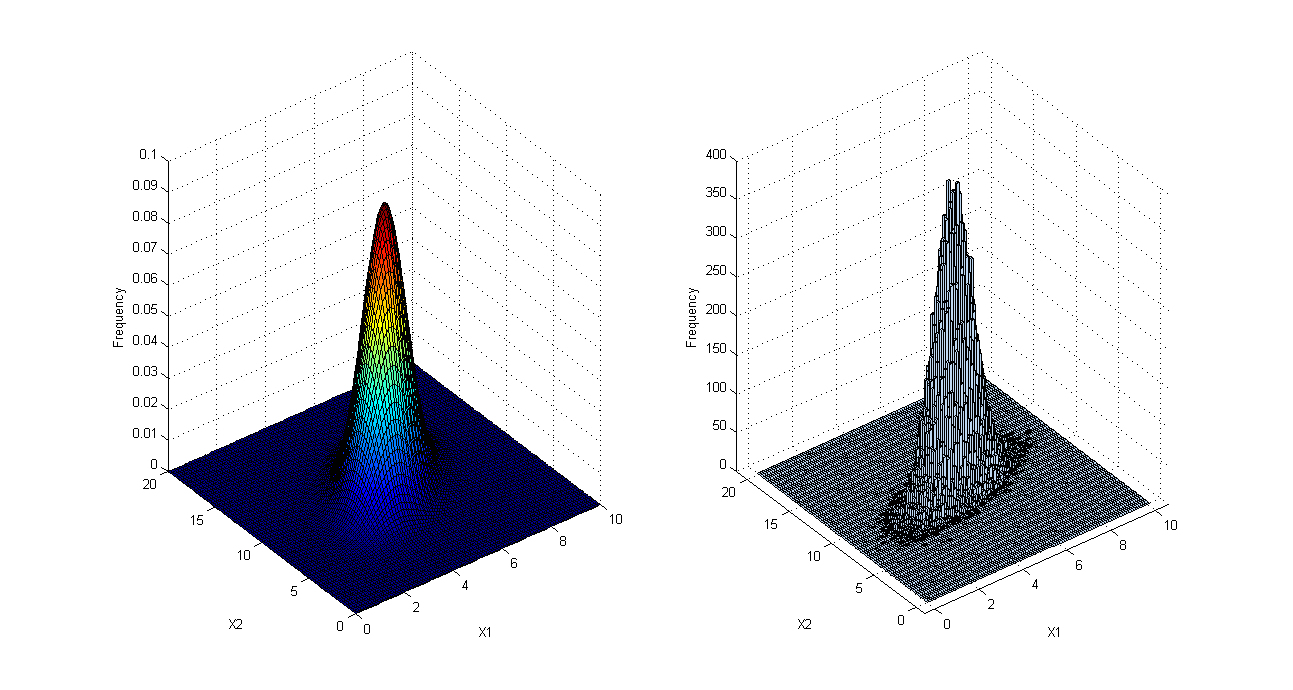
\includegraphics[width=10cm,height=5cm]{Gibbs.png}
    \caption{\scriptsize{Gibbs采样算法生成随机样本}}
    \label{TGibbs}
\end{figure}

\subsection{数值结果与算法比较}

下面对Gibbs采样算法、参数优化之后的Metropolis-Hastings算法、最初实现的MH算法共三种算法在图\ref{MH_Compare}和表\ref{MHGibbsCom}中加以对比。将各种算法独立运行20次,各算法对相关系数估计值的精确度、稳定性和计算效率分别用相关系数均值、相关系数方差和运行时间来表示。

从图\ref{MH_Compare}可以直观地看出参数优化后的MH算法和Gibbs采样算法的精确性和稳定性相当,且都优于未优化的MH算法。

表\ref{MHGibbsCom}则用具体的数据表明,Gibbs算法的准确度、稳定性优于其他两种算法。参数未优化的MH算法估计值的精确度相对较低,稳定性也较差,但计算效率很高;而参数优化后的MH算法估计的准确性和稳定性相对于优化之前有了明显的提高,但是计算时间非常长,效率很低。

\begin{figure}[h]
    \centering
    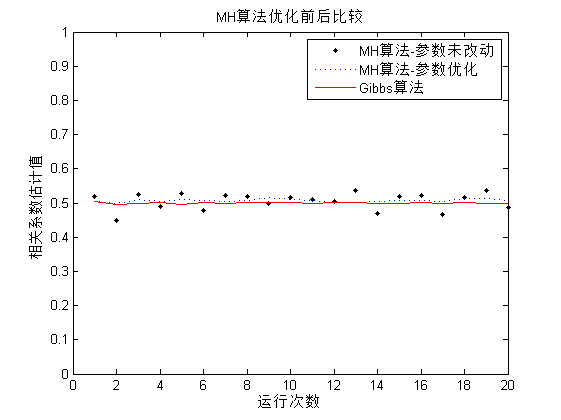
\includegraphics[width=10cm,height=8cm]{MH_Compare.png}
    \caption{\scriptsize{不同算法对相关系数的估计值比较}}
    \label{MH_Compare}
\end{figure}

\begin{table}[tbp]
  \centering  
  \begin{tabular}{lccc} 
  \hline
  算法 & 相关系数均值 & 相关系数方差 & 运行时间\\ \hline
  MH算法(最初实现) & 0.5085 & 4.4757e-04 & 8.152s\\      
  MH算法(参数优化后) & 0.5038 & 8.3389e-06 & 238.573s\\
  Gibbs采样算法 & 0.4998 & 5.7696e-06 & 42.153s\\ \hline
\end{tabular}
\caption{不同算法结果对比}
\label{MHGibbsCom}
\end{table}


\subsection{小结}
Part A对Metropolis-Hastings算法进行了基本实现,并且针对MH算法中各种参数的选取进行了系统而深入地讨论,大大优化了MH算法的计算精确度,但是在计算效率上有所降低。通过生成给定二维高斯的分布随机样本估计相关系数,对优化后的算法和Gibbs算法进行了测试,对估计结果的准确性、稳定性和计算效率进行了对比。结果表明,Gibbs算法的性能最优,参数优化后的MH算法对相关系数估计的精确度和稳定性比优化之前的MH算法明显提高,但计算效率有所降低。

\newpage

\section{Part B: RBM模型归一化常数的估计}
本部分将研究RBM模型归一化常数的估计问题,这一问题随着深度学习的发展受到越来越多的关注\cite{AIS}。如果能够估计得到更加精确的归一化常数,将有助于深度学习等诸多领域的发展。这一部分首先对受限玻尔兹曼机(RBM)进行基本介绍,然后给出三种估计归一化常数的采样算法,包括:AIS(Annealed Importance Sampling)算法,TAP(Thouless-Anderson-Palmer)算法和RTS(Rao-Blackwellized Tempered Sampling)算法。

本文实现并对比了以上算法,并尝试对算法中一些细节进行了补充,最终得到RBM模型的归一化常数,然后根据所得的结果,在测试数据上得到似然值。

\subsection{基本介绍}
\subsubsection{受限玻尔兹曼机模型}
受限玻尔兹曼机(Restricted Boltzmann Machine,RBM)由Hinton和Sejnowski于1986年提出\cite{RBM},该模型由一些可见单元(visible unit,对应可见变量)和一些隐藏单元(hidden unit,对应隐藏变量)构成,可见变量和隐藏变量都是二元变量,亦即其状态取$\{0,1\}$。RBM是一个二部图,只有可见单元和隐藏单元之间存在边,可见单元之间以及隐藏单元之间都没有边连接。

\begin{figure}[h]
    \centering
    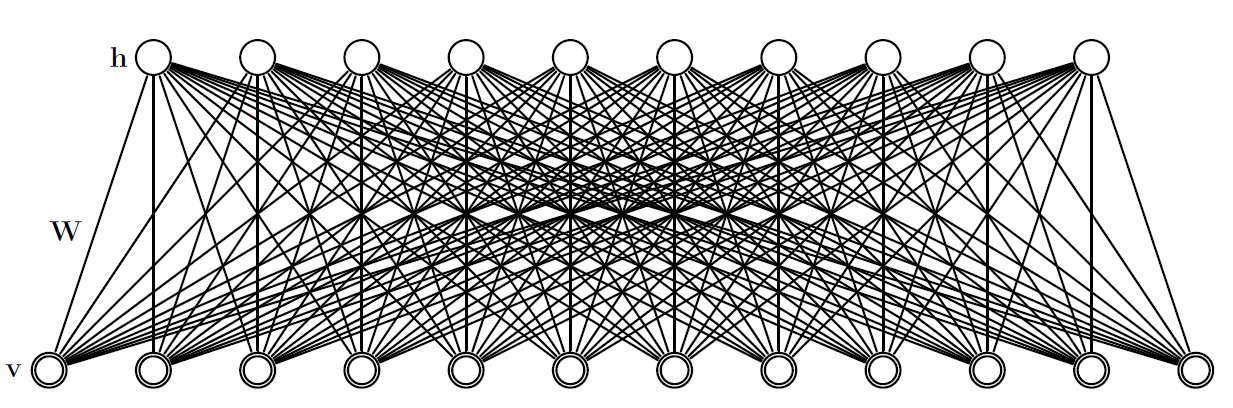
\includegraphics[width = 12cm, height = 4cm]{RBM.png}
    \caption{\scriptsize{受限玻尔兹曼机示意图}}
    \label{RBM}
\end{figure}


\subsubsection{归一化常数及似然值}
RBM在${\mathbf{v},\mathbf{h}}$状态下的能量为
\[E(\mathbf{v},\mathbf{h};\theta) = -\mathbf{v}^{\rm T}W\mathbf{h}-\mathbf{b}^{\rm T}\mathbf{v} - \mathbf{a}^{\rm T}\mathbf{h}\]

其中,$\theta = \{\mathbf{W},\mathbf{b},\mathbf{a}\}$是模型的参数,$\mathbf{W}$是连接可见单元与隐藏单元的权值矩阵,$\mathbf{a}$和$\mathbf{b}$分别是隐藏单元和可见单元的偏置(bias)向量。\cite{AIS}

可见单元与隐藏单元的联合分布为
\[P(\mathbf{v},\mathbf{h};\theta) = \frac{1}{Z(\theta)} exp(-E(\mathbf{v},\mathbf{h};\theta))\]

\[Z(\theta) = \sum_{\mathbf{v}}\sum_{\mathbf{h}} exp(-E(\mathbf{v},\mathbf{h};\theta))\]

\[P(v;\theta)=\frac{1}{Z(\theta)}\sum_{\mathbf{h}}exp(-E(\mathbf{v},\mathbf{h};\theta))\]

其中,$Z(\theta)$就是RBM模型的归一化常数,也称为Partition Function。本部分正是通过不同的算法实现对这一常数的估计。而$P(v;\theta)$表示RBM模型在测试数据$\mathbf{v}$上的似然值。具体计算公式为:

\[P(v;\theta)=\frac{1}{Z(\theta)}exp(\mathbf{b}^{\rm T}\mathbf{v})\prod_{j=1}^{F}(1+exp(a_{j}+\sum_{i=1}^{D}W_{ij}v_{i})).\]

后文提到的在测试数据上的总似然值是指:若测试数据共有$M$个$\mathbf{v}$,则总似然值为
\[P=\sum_{n=1}^{M}P(\mathbf{v}_{n};\theta)\]

事实上,更一般的似然函数常对$P(v;\theta)$取自然对数\cite{AIS},后面的对比给出取log的似然值,此时测试数据上的总似然值(log-likelihood)为

\[L(\theta) = \frac{1}{N}\sum_{n=1}^{N}log(P(\mathbf{v}_{n};\theta)\]


\subsection{Annealed Importance Sampling算法}
\subsubsection{算法描述}
AIS(Annealed Importance Sampling)算法由Radford M. Neal于1998年提出\cite{AIS_O},其核心思路是:使用“中间分布”,从一个已知的简单分布出发,经过一系列中间分布,最终估计得到RBM的归一化常数。算法描述详见Algorithm\ref{RBM_AIS}。

\begin{algorithm}[t]
\caption{AIS算法} 
\begin{enumerate} 
  \item 输出$\beta_{k}$,$0 = \beta_{0}<\beta_{1}<\cdots<\beta{K} = 1$
  
  \item 从$P_{A} = P_{0}$抽样得到$x_{1}$;

  \item \textbf{for}$ k = 1:K-1$ 

  使用Markov转移算子$T_k(\textbf{x}_{k+1}\rightarrow\textbf{x}_{k})$由$\textbf{x}_{k}$抽样得到$\textbf{x}_{k+1}$

  \textbf{end}
 
  \item 令$\omega_{AIS} = \prod_{k = 1}^{K} P_{k}^{*}\textbf{x}_{k}/P_{k-1}^{*}\textbf{x}_{k}$
 
  \item $Z_{B}\approx Z_{A}\frac{1}{M}\sum_{i=1}^{M}\omega_{AIS}^{(i)}$

\end{enumerate} 
\label{RBM_AIS} 
\end{algorithm}

\subsubsection{算法实现}
AIS算法的实现需要以下数据,包括:RBM模型的参数$\theta = \{\mathbf{W},\mathbf{b},\mathbf{a}\}$、用于生成中间分布的$\beta$以及AIS算法的执行次数$M$,还需要选择参考的基准分布(base-rate model)。其中,RBM模型的参数已经给出,是根据训练数据使用相关算法所得。因而,参数$\beta$和$M$是影响AIS算法的两个重要因素。

初步实现AIS算法时,base-rate model的选择越简单越好,因而使用的base-rate model极为简单:$\mathbf{W}$元素全为0,$\mathbf{a}$的元素全为1,$\mathbf{b}$的元素全为0。其他参数使用建议参数:$\beta_{k}$在0至0.5均匀取500个,0.5至0.9均匀取4000个,0.9至1.0均匀取10000个,共计14500个中间分布。AIS算法执行次数$M$选为50次。

以隐变量为10的RBM模型为例,图\ref{RBM_AIS_Origin}展示了AIS算法初步实现的结果,从图中可以看出,当多次独立运行AIS算法时,对R归一化常数的估计值波动很大,表明当前AIS算法的参数选择不太合适,因而需要一定的优化。

\begin{figure}
\begin{minipage}[t]{0.5\linewidth}
    \centering
    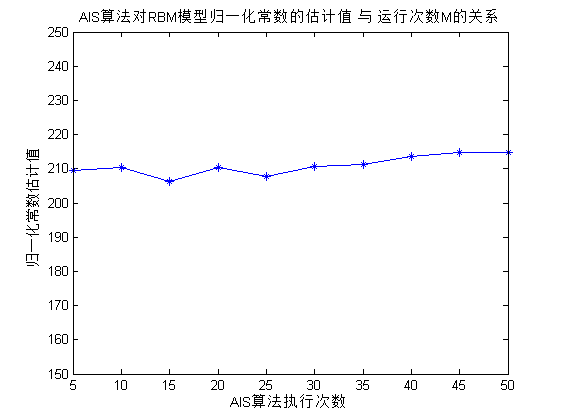
\includegraphics[width=6.5cm,height=5cm]{AIS_Mrun.png}
    \caption{\scriptsize{AIS算法--归一化常数估计值与AIS执行次数的关系}}
    \label{RBM_AIS_Mrun}
\end{minipage}
\begin{minipage}[t]{0.5\linewidth}
    \centering
    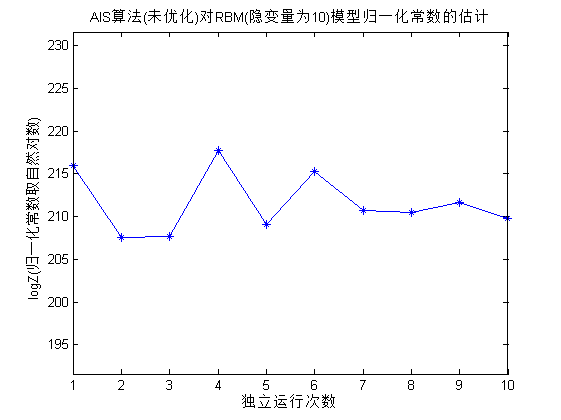
\includegraphics[width=6.5cm,height=5cm]{AIS_Origin.png}
    \caption{\scriptsize{AIS算法初步实现--对隐变量为10的RBM模型的归一化常数估计}}
    \label{RBM_AIS_Origin}
\end{minipage}
\end{figure}

\subsubsection{算法分析和算法优化}
本部分对AIS算法参数的选择进行了细致地对比分析,并根据结论对AIS算法的参数进行优化,同时对base-rate model的选择进行了思考。经过优化之后,归一化常数估计值稳定性明显提高。

\noindent\textbf{a) AIS算法执行次数$M$}

AIS执行次数越多,最终估计得到的结果也越精确和稳定,但是当执行次数足够大时,多余的运行反而会浪费很长时间,降低计算效率。因而,为了兼顾估计值的准确性和计算的效率,现对AIS算法执行次数不同时的估计值结果进行比较,找到既能保证精确性又不会造成太大计算压力的执行次数$M$。

图\ref{RBM_AIS_Mrun}展示了归一化常数估计值与AIS执行次数的关系,可见即使执行次数较低,估计值已经基本接近于稳定值,因而为了提高计算效率,可以适当减小AIS执行次数$M$。


\noindent\textbf{b) $\beta_{k}$的选择}

$\beta$向量用于生成中间分布,$\beta$元素的个数和取值之间影响了中间分布。与执行次数$M$一样,AIS算法同样需要在中间分布数目和计算效率之间加以权衡。同时,$\beta$的取值也需要研究。

\begin{figure}
\begin{minipage}[t]{0.5\linewidth}
    \centering
    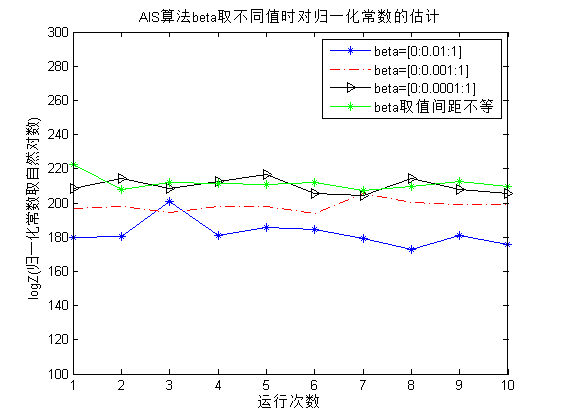
\includegraphics[width=6.5cm,height=5cm]{AIS_Beta.png}
    \caption{\scriptsize{AIS算法--归一化常数估计值与$\beta$取值的关系}}
    \label{RBM_AIS_Beta}
\end{minipage}
\begin{minipage}[t]{0.5\linewidth}
    \centering
    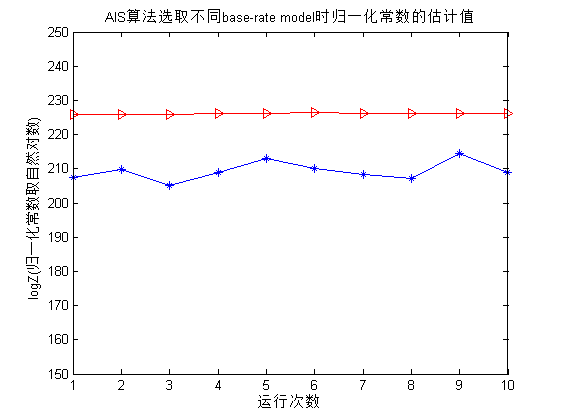
\includegraphics[width=6.5cm,height=5cm]{AIS_Data.png}
    \caption{\scriptsize{AIS算法--base-rate model不同时的归一化常数估计值}}
    \label{RBM_AIS_Data}
\end{minipage}
\end{figure}

图\ref{RBM_AIS_Beta}展示了$\beta$取不同值时对归一化常数的估计(AIS执行次数$M = 10$)。

\noindent\textbf{c) 改变base-rate model}

在之前的实现中,base-rate model都选择了一个非常简单的RBM模型,这一模型的参数与真实的RBM模型相差太大,为了减小base-rate model与实际RBM模型之间的差距,可以使用测试数据的可见层数据生成base-rate model的可见层的偏置向量。

图\ref{RBM_AIS_Data}展示了base-rate model更改前后的对归一化常数的估计值比较。
可以看出,参数优化后的AIS算法的估计值稳定性更好。

\subsubsection{参数优化后的AIS算法}
优化后的参数为:

(1) $M = 20$;

(2) $\beta = [0:1/1000:0.5 0.5:1/10000:0.9 0.9:1/100000:1.0]$;

(3) 使用测试数据的可见层数据生成base-rate model的可见层的偏置向量。

表\ref{AIS_Result}展示了AIS算法的最初实现和优化后的结果对比,可以看出优化后的AIS算法其结果的稳定性明显增强,运行时间也大幅度缩短,说明在结果精确性和计算的效率两方面都得到了提高。

\begin{table}[!htbp]
  \centering  
  \begin{tabular}{lccc} 
  \hline
  算法 & 归一化常数均值 & 归一化常数方差 & 运行时间\\ \hline
  最初实现 & 213.5859 & 14.6869 & 240.246s\\      
  参数优化后 & 226.0064 & 0.0486 & 129.734s\\ \hline
\end{tabular}
\caption{AIS算法优化前后结果对比}
\label{AIS_Result}
\end{table}

\subsection{Thouless-Anderson-Palmer算法}
\subsubsection{算法描述}

TAP(Thouless-Anderson-Palmer)算法,借用了统计物理的思想,通过高阶近似,提出一种计算RBM归一化常数的新思路\cite{TAP}。事实上,TAP算法的本质是不动点迭代法求全局收敛值。TAP算法计算归一化常数时使用了高阶近似,保留的阶数越高,对归一化常数的估计越精确。

\subsubsection{TAP算法(二阶和三阶)实现}
TAP算法的思路比较简单。首先引入了表征可见单元和隐藏单元的向量$\mathbf{m}^{\mathbf{v}}$和$\mathbf{m}^{\mathbf{h}}$,然后$\Gamma$为
$(\mathbf{m}^{\mathbf{v}},\mathbf{m}^{\mathbf{h}})$的函数,通过不动点迭代的方法,$\mathbf{m}^{\mathbf{v}}$和$\mathbf{m}^{\mathbf{h}}$收敛到确定的值,此时$(\mathbf{m}^{\mathbf{v}},\mathbf{m}^{\mathbf{h}})$对应的$\Gamma(\mathbf{m}^{\mathbf{v}},\mathbf{m}^{\mathbf{h}})$即为所求的归一化常数(取自然对数)。

由于$\Gamma$为
$(\mathbf{m}^{\mathbf{v}},\mathbf{m}^{\mathbf{h}})$实际上是近似函数,一般选用二阶和三阶近似,更高阶的近似将会导致计算效率的严重下降。因而,本文实现了TAP算法的二阶近似和三阶近似,并对比两种近似的估计结果。

\subsubsection{算法分析与比较}
现分别对隐变量为10,20,100,500的RBM模型,二阶和三阶TAP算法独立运行多次,得到归一化常数的均值和方差。


\begin{table}[!htbp]
  \centering  
  \begin{tabular}{lcccc} 
  \hline
  隐变量数 & 算法 & 均值 & 方差 & 运行时间\\ \hline
  10 & TAP算法(二阶)& 208.3563 & 89.5157 & 0.010s\\      
  10 & TAP算法(三阶) & 203.9581 & 255.3639& 0.198s\\ \hline
  20 & TAP算法(二阶)& 196.3531 & 92.8964& 0.020s\\      
  20 & TAP算法(三阶) & 199.6899 & 84.9831& 0.676s\\ \hline
  100 & TAP算法(二阶)& 328.2481 & 47.9057 & 18.284s\\      
  100 & TAP算法(三阶) & 334.9081 & 7.6280 & 28.734s\\ \hline
  500 & TAP算法(二阶)& 449.8376 & 0.0697 & 24.284s\\      
  500 & TAP算法(三阶) & 449.9967 & 0.0000& 38.734s\\ \hline
\end{tabular}
\caption{TAP算法二阶近似与三阶近似估计归一化常数对比}
\label{TAP_Result}
\end{table}

从表\ref{TAP_Result}中可以看出因变量数增加时,三阶TAP算法的稳定性比二阶TAP算法的稳定性相对较高。而且从运行时间来看,TAP三阶算法的时间比二阶算法略长一些,计算效率有所降低。

另外,有以下两点值得关注的问题:

a) 即便TAP算法是使用不动点迭代的思想求得收敛值,但是估计得到的归一化常数仍然有一定波动,尤其是对隐藏变量较少的RBM模型,波动十分明显。因而TAP算法对隐藏变量较多的模型优势更加明显一些。

b) 如果使用rand函数生成随机数,那么得到的估计结果波动性很强;但是如果初值确定,得到的估计结果基本保持稳定。


\subsection{Rao-Blackwellized Tempered Sampling算法}
RTS算法的思想和AIS算法有异曲同工之处,同样都运用了中间分布的思想。使用$\{0 = \beta_{1} < \beta_{2} < \cdots < \beta_{K} = 1\}$生成中间分布函数$f_{k}(x)$。$p_{1}(x)$是易于采样的分布函数,而$f(x)$是尚未归一化的目标分布,$p(x\vert\beta_{1}) = p_{1}(x)$,$Z_{K}$即为目标的归一化常数。\cite{RTS}

RTS算法计算归一化常数的式子如下式:
\[ \hat{Z}_{k}^{\rm RTS} = \hat{Z_{k}}\frac{r_{1}}{r_{k}}\frac{\hat{c_{k}}}{\hat{c_{1}}}\]

其中,$\hat{Z_{k}}$是$Z_{k}$的近似值,$r_{k}=r(\beta_{k})$是$\beta_{k}$的先验分布,\cite{RTS}中建议可以选择为均匀分布,即$r_{k} = \frac{1}{K}$。其他参数的计算方法及解释见表\ref{RTS_Formu}

\begin{table}[!htbp]
  \centering  
  \begin{tabular}{cccc} 
  \hline
  公式 & 解释 \\ \hline
  $f_{k}(x) = f(x)^{\beta_{k}}p_{1}(x)^{1-\beta_{k}}$ & 中间分布 \\
  $p(x\vert\beta_{k}) = \frac{f_{k}(x)}{Z_{k}}$ & 条件分布 $x\vert\beta_{k}$ \\ 
  $Z_{k} = \int f_{k}(x)dx$ & 中间分布的归一化常数 \\
  $\hat{c_{k}}=\frac{1}{N}\sum_{i = 1}^{N}q(\beta_{k}\vert x^{(i)})$ & $q(\beta_{k})$的无偏估计\\\hline
\end{tabular}
\caption{对RTS算法参数的解释}
\label{RTS_Formu}
\end{table}

RTS算法可以总结为Algorithm\ref{RTS}.
\begin{algorithm}[t] 
\caption{Rao-Blackwellized Tempered Sampling采样算法} 

\textbf{输入:} $\{\beta_{k},r_{k}\}_{k = 1,\cdots,K}$, N

\textbf{初始化:} $log\hat{Z}_{k},k = 2,\cdots,K$;$\beta\in\{\beta_{1},\cdots,\beta_{K}\}$;$\hat{c}_{k} = 0,k = 1,\cdots,K$

\textbf{输出:} $\hat{Z}_{k}^{\rm RTS}$

\textbf{for} $t=1:N$ 
\begin{enumerate} 
  \item 使用Markov转移算子使得$q(x\vert\beta)$不变;

  \item 从$q(\beta\vert x)$中抽样得到$\beta\vert x$

  \item 更新$\hat{c}_{k} = \hat{c}_{k} + \frac{1}{N}q(\beta_{k}\vert x)$

\end{enumerate} 
\textbf{end}

更新$\hat{Z}_{k}^{\rm RTS} = \hat{Z_{k}}\frac{r_{1}}{r_{k}}\frac{\hat{c_{k}}}{\hat{c_{1}}}, k = 2,\cdots,K$
\label{RTS} 
\end{algorithm}

\subsection{总结}
\subsubsection{三种算法比较}
本文一共实现了AIS、TAP、RTS共三种估计RBM模型归一化常数的算法,每种算法各有优缺点。图\ref{TCompare}和表\ref{Compare}以隐变量为10的RBM模型(对应于h10.mat数据)为例,细致比较了三种算法(TAP算法使用二阶和三阶两种近似)的各运行10次的结果(均值和方差)和运行时间。从图\ref{TCompare}和表\ref{Compare}中可以得到以下结论:

\begin{figure}
    \centering
    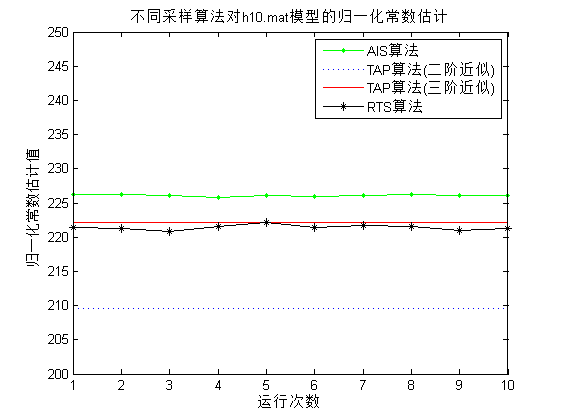
\includegraphics[width=10cm,height=8cm]{Compare.png}
    \caption{不同采样算法对归一化常数的比较}
    \label{TCompare}
\end{figure}

\begin{table}[!htbp]
  \centering  
  \begin{tabular}{cccc} 
  \hline
  算法 & 均值 & 方差 & 运行时间\\ \hline
  AIS算法 & 226.0957 & 0.0122 & 18.639s \\
  TAP算法(二阶) & 209.5460 & 8.9755e-28 & 0.420s\\
  TAP算法(三阶) & 222.1476 & 0  & 0.942s\\
  RTS算法 & 221.4095 & 0.0148 & 12.462s\\ 
  \hline
\end{tabular}
\caption{不同采样算法性能比较}
\label{Compare}
\end{table}

\noindent\textbf{(a)}
AIS的优点是计算结果精确性和稳定性都很高,但是计算时间过长,即计算效率较低。

\noindent\textbf{(b)}
TAP算法整体的计算效率较高,但是计算结果的稳定性相对于AIS较差。并且,三阶近似时比二阶近似的结果稳定好一些,运行时间有所增加。

\noindent\textbf{(c)}
RTS算法的估计结果于AIS相比稳定性较差,但是略优于TAP算法;运行时间比AIS短。

总之,三种算法都存在着“精确性与计算效率”不可兼得的矛盾,因为如果要想得到更加准确稳定的结果,往往需要耗用更长的时间、动用更多的资源来实现这一点。在实际应用中,应当视需要选择合适的算法估计归一化常数。

事实上,由于超级计算机等技术的发展,计算时间已经不再是非常严重的影响因素,因而本文所给出的归一化常数和似然值的结果都是通过AIS算法得到的。

\subsubsection{基本结论}
表\ref{Final_Result}给出了使用AIS算法对四种RBM模型的归一化常数的估计结果\footnote{表中的e-31表示10的-31次方,依次类推。},以及由归一化常数计算的在测试数据test.mat上的总似然值。

\begin{table}[!htbp]
  \centering  
  \begin{tabular}{cccc} 
  \hline
  RBM隐变量数 & 归一化常数估计(取log) & 总似然值 & log-likelihood\\ \hline
  10 & 226.1046 & 1.5272e-31 & -173.8708 \\
  20 & 221.0592 & 9.1561e-21 & -145.1603 \\
  100 & 348.3669 & 8.6656e-14 & -112.8921\\
  500 & 460.1208 & 2.1974e-13 7 & -100.6043\\ 
  \hline
\end{tabular}
\caption{归一化常数估计值和测试数据上的似然值结果汇总}
\label{Final_Result}
\end{table}

\subsection{训练受限玻尔兹曼机}
根据已有的train.mat训练数据,本文尝试使用对比散度(CD, Contrastive Divergence)算法从训练数据中得到不同隐变量数目的RBM模型,再运用之前实现的AIS等算法估计模型归一化常数,并在估计结果上计算出测试数据上的似然值。

\subsubsection{Contrastive Divergence算法}
Contrastive Divergence算法是Hinton在2002年提出了RBM的一种快速学习算法\cite{CD},
有关CD算法,详见Algorithm\ref{CD}。
\begin{algorithm}[t] 
\caption{Contrastive Divergence算法} 

\textbf{输入:} 一个训练样本$x_{0}$;隐藏单元个数$m$;学习率$\epsilon$;最大训练周期T.

\textbf{输出:} 可见层和隐藏层的连接矩阵$\mathbf{W}$,可见层的偏置(bias)向量$\mathbf{a}$、隐层的偏置向量$\mathbf{b}$.

\textbf{训练模型}

\textbf{初始化:} 令可见层单元的初始状态$\mathbf{v}_{1} = \mathbf{x}_{0}$;$\mathbf{W}$、$\mathbf{a}$、$\mathbf{b}$为随机的较小数值。

\textbf{for} $t=1:T$

\textbf{for} $j=1:m$(对所有隐藏单元)
计算$P(\mathbf{h}_{1j} = 1\vert\mathbf{v}_{1}) = \sigma(b_{j}+\sum_{i}v_{1i}\mathbf{W}_{ij})$;从条件分布$P(\mathbf{h}_{1j}\vert\mathbf{v}_{1})$中抽取$h_{1j}\in\{0,1\}$. 
\textbf{end}

\textbf{for} $i=1:n$(对所有可见单元)
计算$P(\mathbf{v}_{2i} = 1\vert\mathbf{h}_{1}) = \sigma(a_{i}+\sum_{j}\mathbf{W}_{ij}h_{1j})$;从条件分布$P(\mathbf{v}_{2i}\vert\mathbf{h}_{1})$中抽取$h_{2i}\in\{0,1\}$.

\textbf{for} $j=1:m$(对所有隐藏单元)
计算$P(\mathbf{h}_{2j} = 1\vert\mathbf{v}_{2}) = \sigma(b_{j}+\sum_{i}v_{2i}\mathbf{W}_{ij})$;
\textbf{end}

按照下式更新各参数:
\begin{enumerate} 
  \item $W  = W+\epsilon(P(\mathbf{h}_{1}=1\vert\mathbf{v}_{1}\mathbf{v}_{1}^{\rm T})-P(\mathbf{h}_{2}=1\vert\mathbf{v}_{2}\mathbf{v}_{2}^{\rm T}))$;

  \item $a = a+\epsilon(\mathbf{v}_{1}-\mathbf{v}_{2})$;

  \item $b  = b+\epsilon(P(\mathbf{h}_{1}=1\vert\mathbf{v}_{1})-P(\mathbf{h}_{2}=1\vert\mathbf{v}_{2})$;
\end{enumerate}

\textbf{end}
\label{CD} 
\end{algorithm}

\subsubsection{训练结果}
本文主要使用MATLAB中的
DeepLearnToolBox\footnote{\url{https://github.com/rasmusbergpalm/DeepLearnToolbox}}对RBM模型进行了训练,得到了隐变量分别为10,20,100,500的RBM模型。使用AIS算法估计训练的模型的归一化常数结果,并计算测试数据上的总似然值,得到表\ref{New_Result}所示的结果。


\subsubsection{对比与分析}
将表\ref{New_Result}与表\ref{Final_Result}的结果对比,发现对于隐变量数目相同的RBM模型,本文训练的结果似然值较低,根据RBM模型最大似然的学习目标,可见已有的RBM模型比自行训练的RBM模型更好。

\begin{table}[!htbp]
  \centering  
  \begin{tabular}{cccc} 
  \hline
  RBM模型的隐变量数 & 归一化常数估计值(取log) & 测试数据上的似然值 \\ \hline
  10 & 188.3565 & 8.2051e-37 \\
  20 & 219.1713 & 1.2873e-29 \\
  100 & 331.8111 & 1.4060e-19 \\
  500 & 442.8689 & 7.0230e-22\\ 
  \hline
\end{tabular}
\caption{ 重新训练RBM模型,归一化常数估计值和测试数据上的似然值结果汇总}
\label{New_Result}
\end{table}

\section{结论}
本文主要讨论了马氏链蒙特卡洛方法的应用,没有提出新的算法,但是在实现算法的过程中,本文也做出了一些比较细致而有新意的工作,优化了算法对参数的估计效果。

第一部分通过马氏链蒙特卡洛方法中的Metropolis-Hastings算法生成了二维高斯分布的随机样本,并且从迭代初值的选取、提议函数的选取、生成随机样本数的选择、判断随机样本收敛以及提高随机样本独立性等五个方面深入讨论了算法中参数选择的原则,从而使得对相关系数的估计值精确性和稳定性明显提高。另外,还实现了Gibbs采样算法,将结果进行了对比分析,得到了一些有价值的结论。

第二部分实现了三种主要的采样算法:AIS、TAP(二阶和三阶)、RTS,对四种RBM模型的归一化常数进行估计,AIS和RTS都用到了马氏链蒙特卡洛方法的基本思想。另外,本文着重对AIS的相关参数也进行了深入的讨论,获得了有价值的结果。最后还尝试使用对比散度(CD)算法训练了RBM,与所给的RBM模型比较,发现自己训练的结果与所给的RBM模型仍有一定差距。

总之,本人尽力完成了力所能及的工作。由于我的学术水平有限,SAMS算法无法按时实现,而且所写文章难免有不足之处,恳请老师和助教批评和指正!


\section{致谢}
历时将近一个月的时间,终于将本次关于马氏链蒙特卡洛的大作业基本完成。本次大作业在阅读文献时,遇到了不少疑问,首先感谢随机过程课程的欧智坚老师和戴音培等助教的耐心解释与帮助,同时也要感谢余东翰、王禹等大神的耐心解答和无私帮助,让我对算法有了比较高层次的认识。最后在自己训练受限玻尔兹曼机时,由于时间比较仓促,所以使用了Rasmus Berg Palm在Github上的DeepLearnToolBox,这一工具箱对我的部分工作起到了很大的帮助。再次,特向以上对我有重要帮助的人表示衷心的感谢!


\newpage
\begin{thebibliography}{1}
\addcontentsline{toc}{section}{参考文献}
\bibitem{UMH}
Chib, Siddhartha, and Edward Greenberg. ``Understanding the metropolis-hastings algorithm." \emph{The American statistician} 49.4 (1995): 327-335.
\bibitem{MH1}
Metropolis, Nicholas, et al. "Equation of state calculations by fast computing machines." \emph{The journal of chemical physics }21.6 (1953): 1087-1092.
\bibitem{Gelman}
Gelman, Andrew, and Donald B. Rubin. "A single series from the Gibbs sampler provides a false sense of security." \emph{Bayesian statistics} 4 (1992): 625-631.
\bibitem{PRML}
Bishop, C. M. ``Bishop Pattern Recognition and Machine Learning." (2001).
\bibitem{Jun}
Liu, Jun S. Monte Carlo strategies in scientific computing. \emph{Springer Science and Business Media}, 2008.
\bibitem{MH_A}
陈平, 徐若曦. Metropolis-Hastings 自适应算法及其应用[J]. 系统工程理论与实践, 2008, 28(1): 100-108.
\bibitem{Lin}
林元烈. 应用随机过程[M]. 清华大学出版社有限公司, 2002.
\bibitem{AIS}
Salakhutdinov, Ruslan. ``Learning deep generative models." Diss. University of Toronto, 2009.
\bibitem{RBM}
Ackley, David H., Geoffrey E. Hinton, and Terrence J. Sejnowski. ``A learning algorithm for Boltzmann machines." \emph{Cognitive science} 9.1 (1985): 147-169.
\bibitem{AIS_O}
Neal, Radford M. ``Annealed importance sampling." \emph{Statistics and Computing} 11.2 (2001): 125-139.
\bibitem{TAP}
Gabrié, Marylou, Eric W. Tramel, and Florent Krzakala. ``Training Restricted Boltzmann Machine via the Thouless-Anderson-Palmer free energy." \emph{Advances in Neural Information Processing Systems.} 2015.
\bibitem{RTS}
Stinson, Patrick, Ari Pakman, and Liam Paninski. ``Partition Functions from Rao-Blackwellized Tempered Sampling."
\bibitem{CD}
Bengio, Yoshua. ``Learning deep architectures for AI." \emph{Foundations and trends® in Machine Learning} 2.1 (2009): 1-127.
\end{thebibliography}


\end{document}
